\documentclass[letterpaper]{article}
\usepackage[utf8]{inputenc}
\usepackage[spanish]{babel}
\usepackage[letterpaper,includeheadfoot, top=.5cm, bottom=3.0cm, right=2.0cm, left=2.0cm]{geometry}
\renewcommand{\familydefault}{\sfdefault}
\usepackage{amsmath}
\usepackage{graphicx}
\usepackage{subcaption}
\usepackage{gensymb}
\usepackage{color}
\usepackage{hyperref}
\usepackage{amssymb}
\usepackage{url}
%\usepackage{pdfpages}
\usepackage{fancyhdr}
\usepackage{enumerate}
\usepackage{enumitem}
\usepackage{float}
\usepackage{tikz}
\usepackage{siunitx}
\usepackage{framed}
\tikzset{
every picture/.append style={
  execute at begin picture={\deactivatequoting},
  execute at end picture={\activatequoting}
  }
}
%-------------------- CABECERA ---------------------
\pagestyle{fancy}
\fancyhf{}
\author{Docente: Martin}
\date{}
\title{\bf Guía 14: Momento Angular}
%Encabezado
\fancyhead[R]{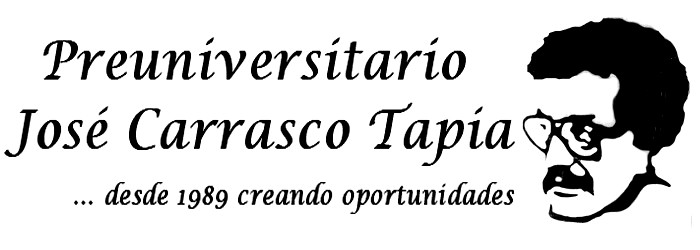
\includegraphics[scale=0.35]{jct.jpg}}
\fancyfoot[C]{\thepage}


\newcommand{\tpb}[1]{node[midway, below, sloped] {#1}}
\newcommand{\tpa}[1]{node[midway, above, sloped] {#1}}
\newcommand{\tvec}[3]{[->, thick] #1 -- #2 \tpb{#3}}
\newcommand{\tveca}[3]{[->, thick] #1 -- #2 \tpa{#3}}
\newcommand{\tvecnotsloped}[3]{[->, thick] #1 -- #2 {node[midway, above] {#3}}}

\newcounter{propiedades}
\newcounter{definiciones}

\newcommand{\propi}{\stepcounter{propiedades} \textbf{Propiedad \thepropiedades}: }
\newcommand{\defii}{\stepcounter{definiciones} \textbf{Definición \thedefiniciones}: }

\newenvironment{prop}
{ \begin{framed} \propi}
{ \end{framed} }
\newenvironment{defi}{\begin{framed} \defii}{\end{framed}}

\renewcommand{\sectionmark}[1]{\markright{\thesection.\ #1}}
\renewcommand{\headrulewidth}{0.5pt}
\renewcommand{\footrulewidth}{0pt}
\setlength{\headheight}{92pt}

% --------------- ---------PORTADA -----------------------
\begin{document}
\maketitle
\thispagestyle{fancy}
\begin{center}
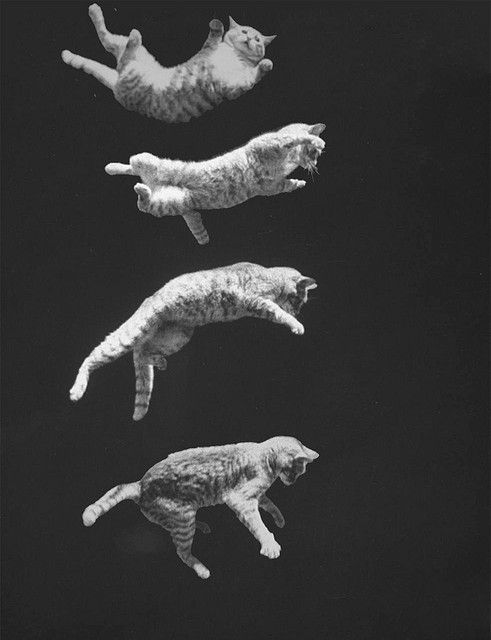
\includegraphics[scale=0.6]{portada.jpg}
\end{center}
\pagebreak

Los egipcios consideraban a los gatos como animales sagrados e incluso les asociaban propiedades mágicas. Cualquier dueño de un gato conoce la ternura de los gatos y la magia de su ronroneos, que pueden levantarte el ánimo incluso en los peores días. Pero los físicos se interesaron mucho en los gatos por otra razón. Por una pregunta que por siglos no conoció respuesta. ¿Cómo es que los gatos siempre caen parados? ¿Cómo es que partiendo del reposo, pueden girar espontáneamente? ¿Nosotros podemos hacer lo mismo? Todo esto y mucho más lo veremos a lo largo de la guía.  

\section*{Fuerzas en MCU}

Recientemente vimos el concepto de fuerzas y cómo pueden explicar el movimiento de una partícula. Hemos visto que en un MCU \emph{siempre} existe una aceleración centrípeta. Aplicando la segunda ley de Newton en un MCU se tiene:
$$\sum \vec{F} = \vec{F}_n = m\vec{a}_c$$

Donde $\vec{F}_n$ representa la fuerza neta sobre la partícula de masa $m$ que describe un $MCU$ de radio $r$ a rapidez tangencial $v$. Por lo tanto, tiene que existir una fuerza neta que apunta hacia el centro de la circunferencia, que llamaremos fuerza centrípeta. Pensemos en el caso del movimiento de la Tierra en torno al Sol que se puede aproximar a un movimiento circular. Ya sabemos que existe una fuerza gravitacional ejercida por el Sol sobre la Tierra que, efectivamente, apunta hacia el centro de rotación de la Tierra (el Sol). Es entonces esta fuerza gravitacional que permite que la Tierra siga un MCU.

\begin{defi}
En un MCU siempre existe una fuerza centrípeta $F_c$ tal que,
$$\vec{F}_c = m\vec{a}_c$$

En particular su magnitud está dada por,
$$|\vec{F}_c| = m|\vec{a}_c| = m\cdot\frac{v^2}{r}$$
\end{defi}

\section*{Fuerza centrífuga}

Probablemente una de las fuerzas más famosas es la que nos bota de las micros cuando giran muy rápido, la que nos permite secar la ropa en la secadora o la que nos empuja hacia afuera en una montaña rusa, así es: la fuerza centrífuga. Paradójicamente, ¡esta fuerza no existe! En física se le llama a este tipo de fuerzas, \emph{fuerzas virtuales} ya que no existen pero aún así se sienten como fuerzas. ¿Cómo se explica esto?


Para comprender el tema tenemos que saber lo que es un sistema inercial. Cuando vimos las leyes de Newton, la verdad es que esas leyes vienen con una letra chica: solo se aplican en un sistema inercial. ¿Qué es un sistema inercial? Pues un sistema en el que se aplican las leyes de Newton. De aquí surge una muy buena pregunta, ¿existe un sistema en donde no se cumplan las leyes de Newton? 

Podemos pensar en el metro, si dejas una maleta con ruedas en reposo en la mitad del metro, las únicas fuerzas que se aplican sobre la maleta son las fuerzas peso, normal, roce estático con el suelo (despreciable porque tiene ruedas) y roce con el aire (también despreciable). Sin embargo, sabemos que la maleta no se mueve verticalmente, por lo tanto, necesariamente la fuerza de peso es igual a la normal, mientras que en el eje horizontal no existe ninguna fuerza, o sea que, por la primera ley de newton, la maleta va a seguir en reposo. En la realidad, cuando el metro comienza a acelerar, la maleta se va al otro extremo del metro ya que se mantiene en reposo respecto a la estación de metro, no al metro en sí. El metro es entonces un sistema no inercial, ya que les las leyes de Newton no se cumplen, mientras que la estación de metro es un sistema inercial.

De manera general, un sistema es no inercial si acelera o rota con respecto a un sistema inercial. En el caso del metro, podemos pensar en la estación de metro como un sistema inercial ya que, efectivamente, las leyes de Newton se cumplen en la estación de metro, y, puesto que el metro está acelerando con respecto a la estación, el metro deja de ser un sistema inercial. Para poder aplicar las leyes de Newton en un sistema no inercial, hay que agregar fuerzas \emph{ficticias} o \emph{virtuales}, como la fuerza centrífuga. De esta manera, para estudiar el movimiento de la maleta, hay que introducir una fuerza ficticia que sería la responsable de que la maleta se escape al otro extremo del metro.                   

\section*{Momento de Inercia}

Dicho simplemente, el momento de inercia es el equivalente de la masa para la rotación de los cuerpos. Cuando estudiamos fuerzas y dinámica vimos que la masa de un objeto es la capacidad que tiene para resistirse al cambio de su movimiento. En el caso de la rotación, es el momento de inercia y no la masa la que determina su resistencia al cambio de movimiento (rotacional). Un ejemplo sencillo es el de la escoba, mientras uno no rompa o separe la escoba en varias partes, su masa va a ser constante lo que implica que al aplicarle la misma fuerza, se va a mover lo mismo. En cambio, si uno quiere rotar la escoba, observará que es más fácil rotar la escoba en torno al eje que pasa por el centro del palo de la escoba. Si se intenta rotar la escoba respecto a un eje perpendicular al palo de la escoba será mucho más difícil. Esto se debe a que el momento de inercia de un cuerpo depende del eje respecto al cual se rota el cuerpo.

\begin{defi}
El momento de inercia de un cuerpo representa su capacidad de resistirse al movimiento de rotación y se determina en función de la repartición de la masa en torno al eje de rotación. Mientras la masa se concentre más cerca del eje de rotación, menor será su momento de inercia, por lo tanto, más fácil será hacerlo rotar. En cambio, si la masa se concentra lejos el eje de rotación, mayor será el momento de inercia y más difícil será hacerlo rotar.

Para un cuerpo puntual, su momento de inercia está dado por:
$$I = mr^2$$

Donde $m$ representa la masa del cuerpo y $r$ la distancia desde el cuerpo hasta el eje de rotación. Se deduce que la unidad del momento de inercia según el \emph{SI} es \si{kg.m^2}.
\end{defi}

Como el momento de inercia depende de la forma del objeto y de la posición del eje de rotación no es necesario conocer el valor asociado a cada forma, solo basta recordar que mientras más lejos esté repartida la masa respecto al eje de rotación mayor será el momento de inercia. En la figura siguiente se puede apreciar el momento de inercia en el caso de algunas formas geométricas.

\begin{figure}[h]
\centering
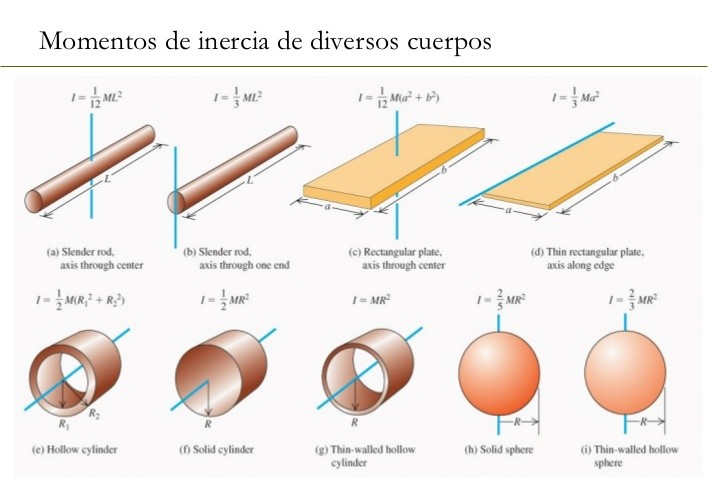
\includegraphics[scale=0.4]{momentos_de_inercia.jpg}
\end{figure}
                        
\section*{Momentum angular}

Así como en cinemática estudiamos el momentum lineal para explicar ciertos fenómenos en un movimiento rectilíneo, ahora estudiaremos el momentum angular para estudiar fenómenos en un movimiento circular. El momentum angular se define de manera análoga al momentum lineal:

\begin{defi}
El momentum angular $\vec{L}$ de una partícula que rota a velocidad angular $\vec{\omega}$ y de momento de inercia $I$, está dado por
$$\vec{L} = I\vec{\omega}$$

Notemos que el momentum angular se expresa en $\si{kg.m^2.s^{-1}}$ de acuerdo al \emph{SI}. 
\end{defi}

Respecto al momentum lineal que en un sistema aislado, donde no actúan fuerzas externas, el momentum lineal se conserva. Ocurre lo mismo para el momentum angular.

\begin{prop}
En un sistema aislado, el momentum angular del sistema se conserva, por lo que podemos escribir:
\begin{align*}
\vec{L}_i &= \vec{L}_f \\
I_i\vec{\omega}_i &= I_f\vec{\omega}_f
\end{align*}
\end{prop}

Podemos observar la conservación de momentum angular en un patinador de hielo artístico, como en la imagen siguiente. En la situación inicial, tiene los brazos extendidos lo que se traduce en un alto momento de inercia. Luego, acerca sus brazos a sí mismo (el eje de rotación) lo que provoca que el momento de inercia disminuya y, por lo tanto, aumente la velocidad angular. Uno puede intentar lo mismo en una silla giratoria para convencerse.

Es importante notar que como el momentum angular es un vector, no sólo su magnitud se mantiene constante en el caso de un sistema aislado, también su dirección y sentido. Sabemos que la dirección y el sentido del momentum angular depende directamente del eje de rotación del sistema, por lo tanto, en un sistema aislado se conserva el eje de rotación.
\begin{figure}[h]
\centering
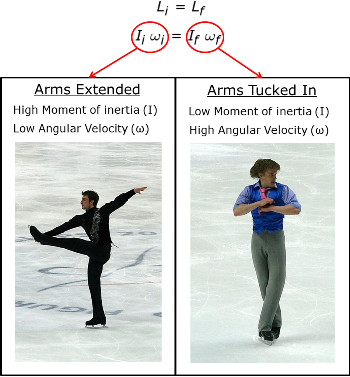
\includegraphics{ang_cons.png}
\end{figure}

Un caso particular es el caso de los gatos que son capaces de girar espontáneamente desde el reposo. Cuando uno deja caer un gato desde el reposo, se pueden pensar como un sistema aislado que comienza con un momentum angular nulo. En la imagen siguiente se representa el movimiento de un gato al caer.

\begin{figure}[h]
\centering
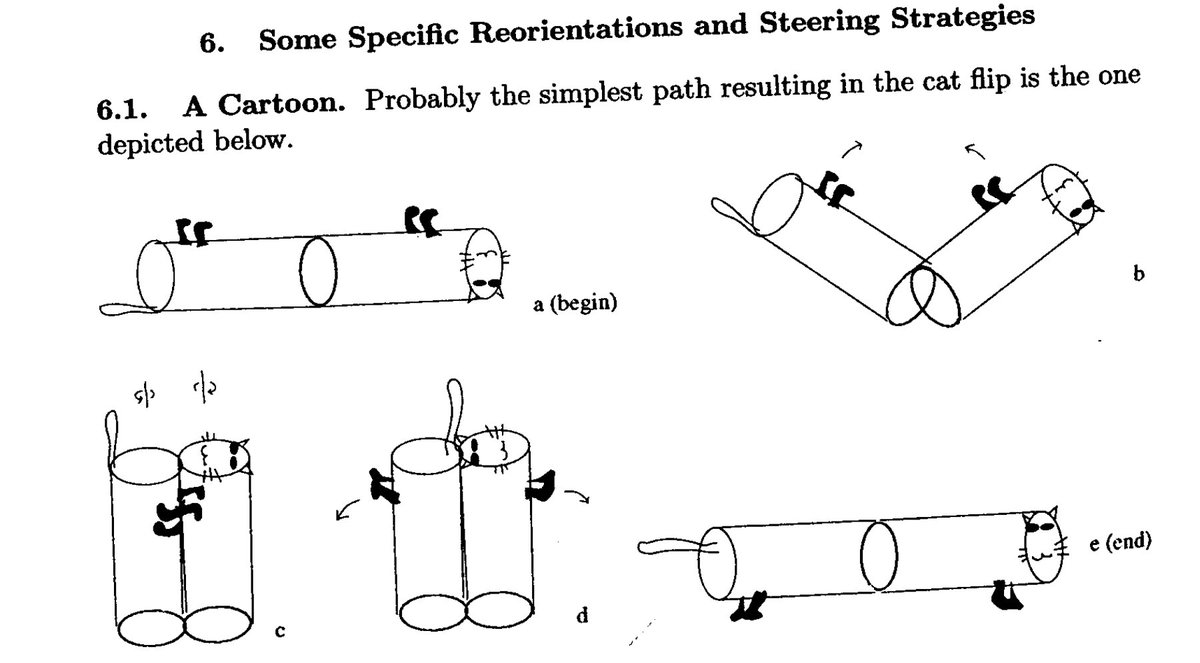
\includegraphics[scale=0.3]{cat.jpg}
\end{figure}

El gato comienza con sus patas hacia arriba, con momentum angular nulo. En la siguiente etapa, curva su espalda para luego poder mover la parte posterior de su cuerpo (la cabeza, las patas delanteras y parte de la columna) en sentido contrario a la parte anterior de su cuerpo (patas traseras, cola y parte de la columna). Finalmente, solo le queda contraer la espalda para llegar al estado final. Claramente la transición de la etapa $c$ a la etapa $d$ le rompería la espalda el gato, es por eso que que esa transición ocurre al mismo tiempo que flecta su espalda.

\section*{Ejercicios}

\begin{enumerate}

\item Una piedra de masa $m$, gira en MCU con una frecuencia $f$ y un radio $R$. Con esta información podemos determinar la magnitud de:

\begin{enumerate}[label=\Roman*)]
\item La aceleración centrípeta
\item La fuerza centrípeta sobre la piedra
\item El momentum angular
\end{enumerate}

\begin{enumerate}[label=\Alph*)]
\item Sólo I
\item Sólo I y II
\item Sólo I y III
\item Sólo II y III
\item Sólo II y III
\item I, II y III
\end{enumerate}

\item Se hace girar una piedra, atada a una cuerda ideal, en un plano horizontal con rapidez constante. ¿Con qué datos podemos calcular la tensión de la cuerda?

\begin{enumerate}[label=\Alph*)]
\item la masa de la cuerda, la frecuencia y el periodo de rotación de la piedra. 
\item la masa, la frecuencia y el periodo de rotación de la piedra.
\item el largo de la cuerda, la masa y el periodo de la piedra.
\item la masa y el largo de la cuerda, y la frecuencia de rotación de la piedra.
\item el peso de la piedra y su frecuencia de rotación
\end{enumerate}

\item Dos cuerpos puntuales $A$ y $B$ describen un MCU. El cuerpo $A$ describe una circunferencia de diámetro $2d$, rota a velocidad angular $\omega$ y tiene una masa $2m$ mientras que el cuerpo $B$ describe una circunferencia de radio $\frac{d}{2}$, rota a velocidad angular $2\omega$ y tiene una masa $m$. Es correcto afirmar que el momento angular de $B$ respecto al de $A$ es

\begin{enumerate}[label=\Alph*)]
\item un medio
\item un cuarto
\item el doble
\item el cuádruple
\item el mismo
\end{enumerate}

\item Un cuerpo es puesto a girar con rapidez constante en una trayectoria circunferencial. Respecto a este objeto se afirma que mientras gira,

\begin{enumerate}[label=\Roman*)]
\item la magnitud de la fuerza centrípeta varía en el tiempo.
\item su velocidad tangencial permanece constante.
\item su frecuencia de rotación es constante.
\end{enumerate}

Es (son) correctas(s)

\begin{enumerate}[label=\Alph*)]
\item sólo I
\item sólo II
\item sólo III
\item sólo I y III
\item sólo II y III
\end{enumerate}

\item Se tienen dos boleadoras hechas con una cuerda ideal y una piedra muy pequeña. La primera tiene una cuerda de largo $\ell$ y una piedra de masa $2m$ mientras que la segunda tiene una cuerda de largo $2\ell$ y una piedra de masa $m$. Es correcto afirmar que el momento de inercia de la piedra de la primera boleadora respecto al momento de inercia de la piedra de la segunda boleadora es 

\begin{enumerate}[label=\Alph*)]
\item el mismo
\item el doble
\item el cuádruple
\item un medio
\item un cuarto
\end{enumerate}

\item Un auto realiza una vuelta U describiendo un MCU por unos instantes. Durante estos instantes, ¿qué fuerza \textbf{no} actúa sobre el auto? 

\begin{enumerate}[label=\Alph*)]
\item Fuerza de roce estático
\item Peso
\item Fuerza centrípeta
\item Fuerza centrífuga
\item Fuerza elástica
\end{enumerate}

\item Un cilindro homogéneo rota con rapidez angular $\omega$ y tienen un momentum angular $L$. Otro cilindro hecho del mismo material, también homogéneo, pero con el doble de masa y el doble de radio, que está girando con una rapidez angular $\frac\omega4$, tendrá un momentum angular de:

\begin{enumerate}[label=\Alph*)]
\item $\frac{L}{4}$
\item $\frac{L}{2}$
\item $L$
\item $2L$
\item $4L$
\end{enumerate}

\item En una batalla espacial, se enfrentan dos naves espaciales, una grande, de forma circular, de momento de inercia $4I$ y radio $200\ \si{m}$ y una pequeña de momento de inercia $\frac{I}{2}$. Desde la tierra se ve que las dos naves están en reposo. A la nave pequeña ya no le quedan recursos para derrotar a la nave grande y prueban una estrategia riesgosa y posiblemente suicida. Es sabido que las naves no pueden soportar una aceleración centrípeta mayor a $10g$ por lo que la nave pequeña decide encender sus motores para alcanzar una rapidez angular $\omega$ tal que, al acoplarse con la nave grande, le transmita parte de su rapidez angular y fuerce la nave grande a rotar tan rápido que no sea capaz de soportar la aceleración centrípeta.
¿Qué rapidez angular ($\omega$) tiene que alcanzar la nave pequeña para que la nave grande sea destruida luego de acoplarse?

\begin{enumerate}[label=\Alph*)]
\item $3\ \si{rad.s^{-1}}$
\item $4\ \si{rad.s^{-1}}$
\item $5\ \si{rad.s^{-1}}$
\item $8\ \si{rad.s^{-1}}$
\item $9\ \si{rad.s^{-1}}$
\end{enumerate}

\item Si la masa de una partícula, que se mueve con MCU, se reduce a la mitad y su radio de giro se cuadruplica manteniendo constante su velocidad angular. Entonces, su momento angular respecto al eje de giro se

\begin{enumerate}[label=\Alph*)]
\item duplica.
\item triplica.
\item cuadriplica.
\item hace 8 veces mayor.
\item hace 32 veces mayor.
\end{enumerate}

\item Un bloque de una tonelada amarrado a una cuerda gira con un periodo de rotación de $10\pi\ \si{s}$ en una trayectoria circular de radio $2\ \si{m}$ en un plano horizontal sin roce. ¿Cuál es la magnitud de la tensión sobre la cuerda?

\begin{enumerate}[label=\Alph*)]
\item $400\ \si{N}$
\item $200\ \si{N}$
\item $80\ \si{N}$
\item $40\ \si{N}$
\item $20\ \si{N}$
\end{enumerate}

\item Una persona está sentada en una silla giratoria con sus extremidades extendidas perpendicularmente al eje de rotación. Luego, abraza sus piernas en posición fetal. Con respecto a lo anterior, se puede afirmar que

\begin{enumerate}[label=\Alph*)]
\item su momentum angular disminuye.
\item su momento de inercia aumenta.
\item su rapidez angular disminuye.
\item su momento de inercia se mantiene constante.
\item su rapidez angular aumenta.
\end{enumerate}

\item Andrea está sentada en un juego en el Parque O'Higgins que consiste en una plataforma giratoria. Sus amigos hacen rotar la plataforma para que alcance una cierta velocidad angular, se desprecia el efecto del roce sobre la plataforma. Andrea decide caminar hacia el centro de la plataforma. Respecto al sistema compuesto por la plataforma y Andrea, se observa que,

\begin{enumerate}[label=\Alph*)]
\item $L$ y $\omega$ disminuyen.
\item $L$ y $\omega$ aumentan.
\item $\omega$ disminuye y $L$ aumenta.
\item $L$ se mantiene constante y $\omega$ disminuye.
\item $L$ se mantiene constante y $\omega$ aumenta.
\end{enumerate}

\item Un alambre rígido se hace rotar en torno a un eje perpendicular al alambre y que pasa por su centro. Luego, se hace rotar en torno a uno de sus extremos. Para mantener el mismo momentum angular en las dos situaciones se tendría que, en la segunda situación,

\begin{enumerate}[label=\Alph*)]
\item aumentar la rapidez angular.
\item aumentar la frecuencia de rotación.
\item disminuir el periodo de rotación.
\item disminuir la frecuencia de rotación.
\item mantener el periodo de rotación.
\end{enumerate}

\item Un patinador de hielo artístico realiza un truco que consiste en hacer una T con su cuerpo, como en la imagen siguiente. Después, se endereza y alinea completamente su cuerpo con el eje de rotación formando una linea recta que coincide con el eje de rotación.

\begin{figure}[h]
\centering
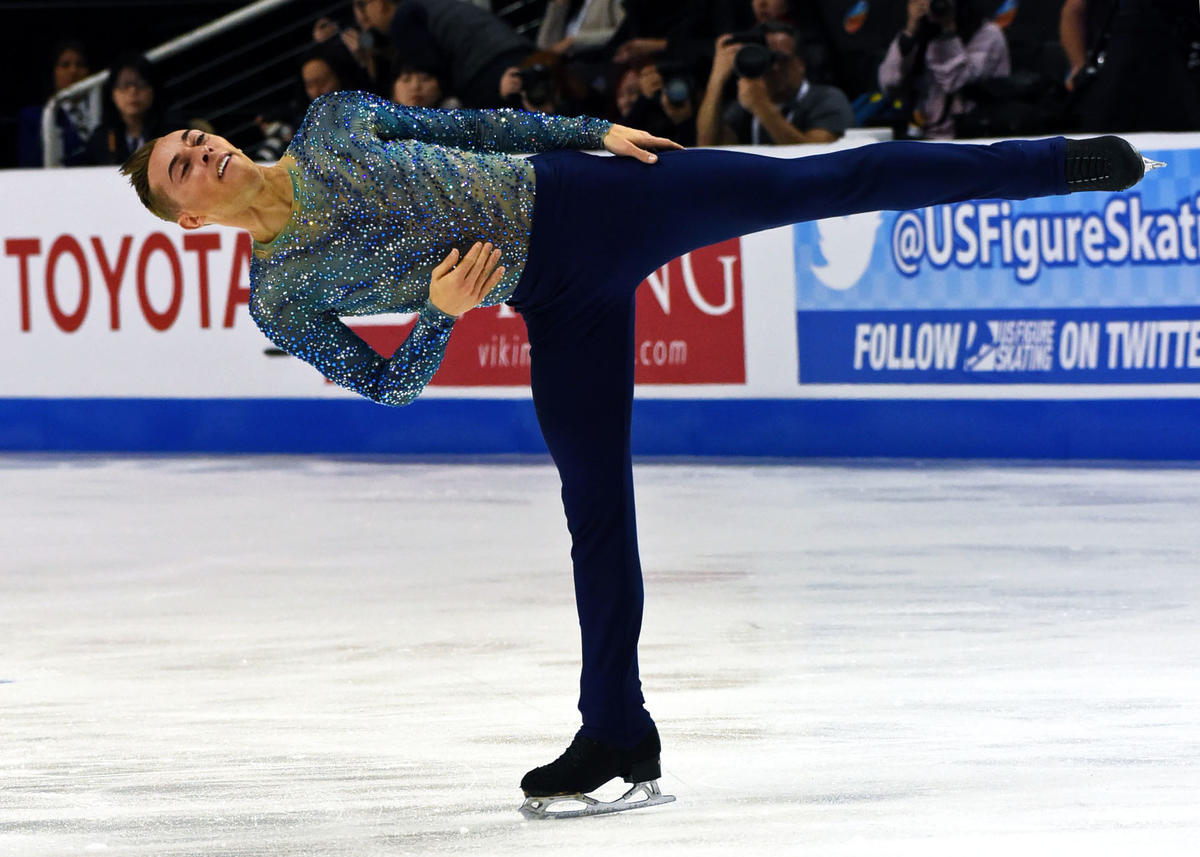
\includegraphics[scale=0.3]{adam.jpg}
\end{figure}

Podemos afirmar que al enderezarse,

\begin{enumerate}[label=\Alph*)]
\item Su momentum angular aumenta.
\item Su momento de inercia aumenta.
\item Su momentum angular disminuye.
\item Su rapidez angular disminuye.
\item Su momento de inercia disminuye.
\end{enumerate}

\end{enumerate}

\vspace{3cm}

\begin{center}
\begin{tabular}{|c|c|c|c|c|}
\hline
 1 & 2 & 3 & 4 & 5 \\ \hline
 B & C & B & C & D \\ \hline
 6 & 7 & 8 & 9 & 10 \\ \hline
 D & D & E & D & C \\ \hline
 11 & 12 & 13 & 14 & 15 \\ \hline
 E & E & D & E & / \\ \hline

\end{tabular}
\end{center}



\section*{Problemas}

\begin{enumerate}

\item Para la difusión de canales de televisión satelital se utilizan los llamados satélites geoestacionarios. La particularidad de estos satélites es que giran junto con la tierra, en otras palabras, siempre están sobre el mismo punto de la Tierra. Determina la altura sobre la superficie de la tierra a la que se debe encontrar un satélite para que sea geoestacionario.

\emph{Nota}: Puede ser útil recordar la ley de gravitación universal.

\item Estrellas bastante más masivas que el Sol, del orden de $10$ veces la masa del sol, pueden transformarse en estrellas de neutrones luego de un colapso gravitacional una vez que ya no les queda más combustible. Gran parte de la masa se pierde en una supernova formando una estrella de neutrones de entre $1,5$ y $3$ masas solares. Típicamente estas estrellas tienen un radio muy muy pequeño, de alrededor de $20\ \si{km}$. 

Tomemos una estrella de $10$ masas solares, de radio del orden de $10^7\ \si{km}$ y velocidad tangencial $30\ \si{km}{s}$ que colapsa gravitacionalmente produciendo una supernova en la que se expulsan $8$ masas solares, dejando una estrella de neutrones de radio $20\ \si{km}$. ¿Cuántas vueltas por segundo da la estrella de neutrones?

\end{enumerate}

\end{document}